<a% !TEX root =  master.tex
\tikzstyle{block} = [rectangle, draw, fill=blue!20, text width=6em, text centered, minimum height=3em]
\tikzstyle{greenblock} = [ellipse, draw, fill=green!20, text width=4em, text centered, minimum height=3em]
\chapter{Codierungstheorie}
Da im Rahmen dieser Arbeit ein kryptographisches Verfahren entwickelt wird, das auf Elementen der Codierungstheorie basiert, wird diese nun zunächst in Definitionen und Hintergründen dargestellt.
\section{Übermittlung von Informationen}
Sowohl in der Kryptographie, als auch in der Codierungstheorie fungieren \textbf{Nachrichten}, die über mit bestimmten Eigenschaften behaftete \textbf{Kanäle} übertragen werden, als die Objekte der Anschauung.
\begin{definition}\label{Alphabet}
Eine \textbf{Nachricht} $m$ sei definiert als eine endliche Folge von Zeichen $a_i \in \Sigma$, wobei $\Sigma$ eine endliche Menge von Zeichen (genannt \textbf{Alphabet}) bezeichnet.
\[m = \langle a_1, a_2, ..., a_{n-1}, a_n \rangle \quad \forall i = 1, ..., n: a_i \in \Sigma\]
\end{definition}
Ein typisches Alphabet sind die Zeichen der \textit{ASCII}-Kodierung, mit denen nahezu alle Worte und Sätze der natürlichen englischen Sprache gebildet werden können \parencite[vgl. ][]{rfc20}. Dieses Alphabet besteht nun nicht aus Zeichen der natürlichen Sprache, sondern aus 7 Bit langen Zahlenwerten, was die Anwendung von Codes oder kryptographischen Verfahren ermöglicht. Im Rahmen dieser Arbeit wird angenommen, dass Zeichen stets in einem Zahlenformat repräsentiert werden. \\\\
Die Definition einer informationstheoretischen Nachricht impliziert eine Autorenschaft, folglich muss jeder Nachricht eine Partei (ein natürliche Person, ein System oder ein Dienst) zugeordnet werden können, die im Folgenden als \textbf{Sender}\footnote{Da sich die Anwendung der modernen Kryptographie sehr überwiegend mit dem Austausch von verschlüsselten Nachrichten zwischen Systemen und nicht unmittelbar zwischen natürlichen Personen befasst, wird hier die männliche Form verwendet (Sender = Dienst/System).} der Nachricht bezeichnet wird. \\
Wird diese Nachricht nun über einen Kanal an eine andere Partei übertragen, so nennen wir diese den \textbf{Empfänger}. Entgegen der in der Kryptographie üblichen \textit{Alice-Bob}-Notation wird in dieser Arbeit diese Terminologie beibehalten, um an den codierungstheoretischen Hintergrund anzuknüpfen. \\\\
Ein \textbf{Kanal} bezeichne ein Medium zur Datenübertragung wie beispielsweise einen elektrischen Leiter, einen Lichtwellenleiter oder die Luft für eine drahtlose Verbindung. Es gibt Kanäle, die Informationen \textbf{digital} übertragen, also als diskrete Binärwerte, und im Gegensatz dazu Kanäle, die fortlaufend und stetig Signale übertragen \parencite[vgl. ][S. 1]{Borda2011}.
\textbf{Rauschen} bezeichne nicht-deterministische Daten, die Nachrichten bei einer Übertragung über einen Kanal unbeabsichtigt hinzugefügt werden und so die Nachricht verändern, sie folglich mit \textbf{Fehlern} versetzen \parencite[vgl. ][S. 1]{vanLint1973}. 
\begin{definition}
Ein \textbf{Kanal} $K$ mit der Menge der Eingabewerte $I$ und der Menge der Ausgabewerte $J$ sei definiert als Matrix 
\[K_{ij} = \textnormal{Pr}(j \mid i) \quad i \in I, j \in J\]
wobei $\textnormal{Pr}(j \mid i)$ definiert sei als die Wahrscheinlichkeit für die Ausgabe $j$ unter der Bedingung $i$. \\\\
Sofern mindestens ein Koeffizient der Matrix $i \neq j$ einen Wert $> 0$ aufweist, ist der Kanal \textbf{rauschend} \parencite[vgl. ][S. 73f.]{Biggs08}.
\end{definition}
\begin{example}
Ein \textbf{\ac{BSC}} $\Gamma$ mit einer Bitfehlerwahrscheinlichkeit $e$ ist definiert durch 
\[\Gamma = \left( \begin{matrix} \Gamma_{00} & \Gamma_{01} \\ \Gamma_{10} & \Gamma_{11}\end{matrix}\right) = \left( \begin{matrix}1 - e & e \\ e & 1 - e\end{matrix}\right)\]
\end{example}

Dass ein Kanal eine Nachricht ohne Rauschen überträgt, ist zwar ein erstrebenswerter Zustand, praktisch jedoch aufgrund der Physik nicht zu erreichen. Jede physische Datenübertragung verläuft nicht fehlerfrei, weshalb die Beziehung $m = m'$ daher nur in einem theoretischen Idealfall gilt. Diese Feststellung liefert die Begründung für die Beschäftigung mit der Codierungstheorie.
\begin{figure}[h!]
\centering
\begin{tikzpicture}[node distance = 1cm and 2cm]
\node[greenblock] (Sender) {Sender};
\node[draw, circle, right = of Sender] (Kanal) {Kanal};
\node[above= of Kanal] (N) {Rauschen};
\node[greenblock, right = of Kanal] (Empf) {Empfänger};
\draw[-] (Sender) -- node[midway, above] {$m$} (Kanal);
\draw[->] (Kanal) -- node[midway, above] {$m'$} (Empf);
\draw[->] (N) -- (Kanal);
\end{tikzpicture}
\caption{Gegenstand der Codierungstheorie (nach \parencite[][S. 1]{Willems2008})}
\label{Gegenstand}
\end{figure}

\section{Problemstellung und Zielsetzung}
Da die Datenübertragung über eine Vielzahl von Kanälen eben nicht fehlerfrei verläuft, liegt es nahe, die Daten so zu übertragen, dass fehlende Bits aus dem Rest der Nachricht erschlossen werden können, wie es zum Beispiel bei natürlicher Sprache der Fall ist. Unsere Worte enthalten häufig Buchstaben, die nicht zwingend erforderlich sind, um das gemeinte Wort zu erkennen \parencite[vgl. ][S. 3]{vanLint1973}. \\\\
Überträgt man diese Erkenntnis auf Nachrichten einer beliebigen Sprache, so lassen sich auch im allgemeinen Fall durch das Hinzufügen von redundanten Informationen Nachrichten erzeugen, deren Informationsgehalt sich auch nach der Übermittlung nicht verringert hat. Ein spezieller Typ dieser Verfahren wird als \textbf{fehlerkorrigierende Codes} bezeichnet \parencite[vgl. ][S. 3]{vanLint1973}. Diese Codes sind dem Gebiet der \textbf{Kanalcodierung} zuzurechnen, die das Ziel hat, die Qualität der Übertragung auf verlustbehafteten Kanälen sicherzustellen. Sie grenzt sich ab von der \textbf{Quellencodierung}, die Verfahren bündelt, welche die Transformation der zu versendenden Daten zum Ziel hat, beispielsweise zur Kompression und Redundanzverringerung \parencite[vgl. ][S. 1]{Manz2017}. Der Fokus dieser Arbeit liegt dabei auf der Kanalcodierung, da die betrachteten kryptographischen Verfahren auf ihr basieren.
\section{Kanalcodierung}
Die Relevanz der Frage, wie möglichst viele Übertragungsfehler in einer Datenübertragung vermieden oder korrigiert werden können, stieg mit der Verbreitung von \acs{EDV}-Systemen und nicht zuletzt dem Internet rasant an \parencite[vgl. ][S. 209]{Borda2011}. Populäre Beiträge der Grundlagenforschung wie jener von \textsc{\citeauthor{Hamming1950}} sind daher auch trotz ihres einige Dekaden umspannenden Alters Fundament der folgenden Definitionen.
\subsection{Grundbegriffe}
Um Codier- und Decodiervorgänge beschreiben zu können, ist eine Erweiterung und Präzisierung der Abbildung \ref{Gegenstand} erforderlich. Die Zuordnung eines Codewortes $c$ zu einer Nachricht $m$ wird als \textbf{Codierung} (der Nachricht) bezeichnet. \\
\begin{figure}[h!]
\centering
\begin{tikzpicture}
[node distance = 1cm, label={ITS}]
\node[greenblock] (S) {Sender};
\node[block, right = of S] (C) {Codierung};
\node[draw, circle, right= of C] (K) {Kanal};
\node[block, right = of K] (D) {Decodierung};
\node[greenblock, right= of D] (E) {Empfänger};
\node[above= of K] (N) {Rauschen};
\draw[->] (S) -- node[midway, above] {$m$} (C);
\draw[->] (C) -- node[midway, above] {$c$} (K);
\draw[->] (K) -- node[midway, above] {$c'$} (D);
\draw[->] (D) -- node[midway, above] {$m'$} (E);
\draw[->] (N) -- (K);
\end{tikzpicture}
\caption{Vereinfachte Darstellung eines \ac{ITS} (nach \parencite[][S. 3]{Borda2011})}
\label{ITS}
\end{figure}

\begin{definition}
Sei $A$ ein Alphabet und $n \in \mathbb{N}$. \\ 
Dann sei $A^{n}$ die Menge aller $n$-Tupel der Form $A^{n} = \lbrace \langle a_1, a_2, ..., a_n \rangle \mid a_i \in A \rbrace$.  \\\\
Ein \textbf{Blockcode} $C$ der Länge $n$ über dem Alphabet $A$ ist definiert als $C \subseteq A^{n} \text{, wobei } \lvert C \rvert > 0$ gelten muss.\\\\
Ist $m = \lvert C \rvert$ und $B$ mit $\lvert B \rvert < m$ die Menge zu codierender Informationseinheiten über einem Alphabet $A'$, so ist jede injektive Abbildung $f\colon B \to C$ eine \textbf{Codierfunktion} \parencite[vgl. ][S. 10]{Manz2017}.
\end{definition}
Neben Blockcodes können auch sogenannte \textbf{Faltungscodes} zur Fehlerkorrektur verwendet werden. Hierbei werden die Informationen nicht unabhängig voneinander blockweise codiert, sondern über Schieberegister in Abhängigkeit zueinander, wodurch sich eine bessere Performanz im Gegensatz zu Blockcodes ergibt \parencite[vgl. ][S. 752]{Viterbi1971}. Der Ansatz, Daten blockweise oder als Datenstrom über Schieberegister zu codieren, weist Parallelen zur kryptographischen Unterscheidung zwischen Block- und Stromchiffren auf. Der Fokus dieser Arbeit wird aufgrund der kryptographischen Bedeutung auf Blockcodes liegen. \\\\
Als Maß der Qualität einer Übertragung beziehungsweise der Verfälschung einer Nachricht durch Rauschen, aber auch für die Unterscheidbarkeit von Codeworte, bietet sich die \textbf{Hamming-Distanz} an.
\begin{definition}
Seien $a = \langle a_1, a_2, ..., a_n \rangle$, $b = \langle b_1, b_2, ..., b_n \rangle \in A^n$ und $A$ ein Alphabet, so ist die \textbf{Hamming-Distanz} $d$ von zwei Codeworten $a$ und $b$ definiert als die Anzahl der abweichenden Stellen in $a$ und $b$:
\[d(a, b) = \lvert \lbrace i \mid 1 \leq i \leq n, a_i \neq b_i \rbrace \rvert\]
Des Weiteren sei die \textbf{Minimaldistanz} eines Blockcodes $C$ mit $\lvert C \rvert > 1$ definiert als 
\[d(C) = \min \lbrace d(x, y) \mid x, y \in C, x \neq y \rbrace\] \parencite[vgl. ][S. 11]{Manz2017} \parencite[vgl. ][S. 105]{Roman1992} \parencite[vgl. ][S. 155]{Hamming1950}.
\end{definition} 
\begin{example}
Seien $A = \lbrace 0, 1 \rbrace$ und $n = 5$. Dann ist $A^n = \lbrace \langle 0, 0, 0, 0, 0\rangle, \langle 0, 0, 0, 0, 1 \rangle , ..., \langle 1, 1, 1, 1, 1 \rangle \rbrace$. Dann gilt für einen Blockcode $C$:
\begin{itemize}
\item $C = A^n \quad \rightarrow \quad d(C) = 1$
\item $C = \lbrace \langle 0, 0, 0, 0, 1 \rangle , \langle 0, 0, 0, 1, 0 \rangle , ..., \langle 1, 0, 0, 0, 0\rangle\rbrace \quad \rightarrow \quad d(C) = 2$
\item $C = \lbrace \langle 0, 1, 0, 1, 0 \rangle , \langle 1, 0, 1, 0, 1 \rangle \rbrace \quad \rightarrow \quad d(C) = 5$
\end{itemize}
\end{example}
Wenn die Werte einer Codierungsfunktion im Bildbereich weit verstreut sind, der Code also eine große Minimaldistanz aufweist, werden die einzelnen Codeworte unterscheidbarer. Folglich ergibt sich aus der Minimaldistanz ein relevantes Kriterium für die Eigenschaft eines Codes, \textbf{fehlererkennend} oder sogar \textbf{fehlerkorrigierend} zu sein. Sie beeinflusst, wie viele Fehler erkannt beziehungsweise korrigiert werden können \parencite[vgl. ][S. 155]{Hamming1950}. \\\\
\textsc{\citeauthor{Hamming1950}} nutzt für seine Argumentation in \parencite{Hamming1950} eine geometrische Betrachtung:
\begin{definition}
Sei $B$ eine Kugel mit Radius $r \geq 2$ und Mittelpunkt $x \in A^n$. Dann liegen alle $a_i \in A^n$ mit $d(a_i, x) = r$ auf der Kugeloberfläche von $B$. Sei $C \subseteq A^n$ nun ein Blockcode mit $d(C) = r$ und $x \in C$. Dann liegen alle $c \in (C \setminus \lbrace x \rbrace )$ auf der Kugeloberfläche oder außerhalb der Kugel $B$. 
\end{definition}
\begin{note}Ein Punkt $a_j \neq x$ mit $d(a_i, x) < r$ (unterscheidet sich in in weniger als $r$ Stellen von $x$) liegt nicht auf der Kugeloberfläche und kann folglich kein fehlerfreies Codewort sein. Ein Code $C$ mit Minimaldistanz $2$ ist damit \textbf{fehlererkennend} für maximal ein falsch übertragenes Zeichen (notiert: {\glqq}1-fehlererkennend{\grqq}). \\\\
Ferner ist ein Code $C'$ mit Minimaldistanz $3$ \textbf{fehlerkorrigierend}: Sei $a_r$ ein gültiges Codewort mit einer Minimaldistanz von $3$ zu allen anderen Codeworten in $C'$. Für ein in einer Stelle abweichendes Wort $a_f$ gilt folglich $d(a_r, a_f) = 1$, aber $\forall a_i \in C' \setminus \lbrace a_r, a_f \rbrace : d(a_i, a_f) > 1$. Damit lässt sich $a_f$ eindeutig $a_r$ zuordnen, wodurch sich der Fehler korrigieren lässt und $C'$ \textbf{1-fehlerkorrigierend} ist \parencite[vgl. ][S. 155f.]{Hamming1950}.
\end{note}
Die Eigenschaft eines Codes, fehlererkennend oder fehlerkorrigierend zu sein, ist skalierbar: 
\begin{definition}
Seien $c, c' \in C; c \neq c'$ Codeworte eines Blockcodes $C \in A^n$, $\epsilon \in \mathbb{N}$, $B_e(c) = \lbrace x \in A^n \mid d(x, c) \leq \epsilon \rbrace$ und $B_e(c')$ analog $B_e(c') = \lbrace x \in A^n \mid d(x, c') \leq \epsilon \rbrace$. \\Dann ist $C$ \textbf{$\epsilon$-fehlerkorrigierend}, wenn $\forall c, c' \in C: B_e(c) \cap B_e(c') = \emptyset$ gilt \parencite[vgl. ][S. 12f.]{Manz2017}.
\end{definition}
\begin{figure}[h!]
\centering
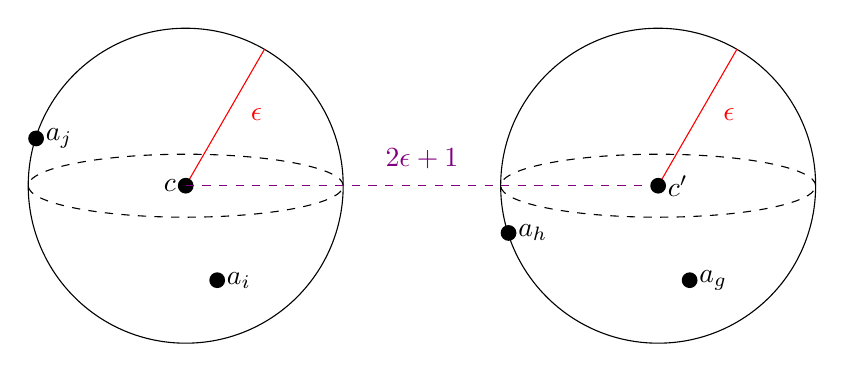
\begin{tikzpicture}[scale=2]
\draw (0,0) circle(1);
\draw[dashed] (0,0) ellipse (1 and .2);
\draw[-, color=red] (0,0)--(.5,0.866);
\draw[color=red] (.45,.45) node {$\epsilon$};
\fill[black] (0, 0) circle (0.05 cm) node[anchor=east]{$c$};
\fill[black] (0.2, -0.6) circle (0.05 cm) node[anchor=west]{$a_i$};
\fill[black] (-0.95, 0.3) circle (0.05 cm) node[anchor=west]{$a_j$};

\draw[dashed, color=violet] (0,0) -- (3, 0);
\draw[color=violet] (1.5, 0.17) node {$2\epsilon + 1$};

\draw (3,0) circle(1);
\draw[dashed] (3,0) ellipse (1 and .2);
\draw[-, color=red] (3,0)--(3.5,0.866);
\draw[color=red] (3.45,.45) node {$\epsilon$};
\fill[black] (3, 0) circle (0.05 cm) node[anchor=west]{$c'$};
\fill[black] (3.2, -0.6) circle (0.05 cm) node[anchor=west]{$a_g$};
\fill[black] (2.05, -0.3) circle (0.05 cm) node[anchor=west]{$a_h$};
\end{tikzpicture}
\caption{Visualisierung der Kugelinterpretation (nach \parencite{Hamming1950})}
\end{figure}
\begin{note}
Ein Blockcode $C$ ist $\epsilon$-fehlerkorrigierend, wenn $d(C) \geq 2 \cdot e + 1$ gilt \parencite[vgl. ][S. 12f.]{Manz2017}.
\end{note}
\begin{definition}
Sei $c \in C$ Codewort eines Blockcodes $C \in A^n$ und $B_t(c) = \lbrace x \in A^n \mid d(x, c) \leq t \rbrace$ die zu $c$ gehörige Kugel mit allen Elementen aus $A^n$, die höchstens $t$ entfernt sind. \\
Dann ist $C$ \textbf{$t$-fehlererkennend}, wenn $\forall c \in C: B_t(c) \cap (C \setminus \lbrace c \rbrace ) = \emptyset$, die Kugel um $c$ also keine anderen Codeworte enthält \parencite[vgl. ][S. 13]{Manz2017}.
\end{definition}
\begin{note}
Ein Blockcode $C$ ist $t$-fehlererkennend, wenn $d(C) \geq t + 1$ gilt \parencite[vgl. ][S. 13]{Manz2017}.
\end{note}
\begin{example}
Sei $A = \lbrace 0, 1 \rbrace$ und $A^3 = \lbrace \langle 0, 0, 0 \rangle , \langle 0, 0, 1 \rangle , ..., \langle 1, 1, 1 \rangle \rbrace$. Ferner sei $C \in A^3$ ein Blockcode für Nachrichten der Form $m = \langle m_1, m_2 \rangle$ mit der Codierfunktion $f\colon M \to C, \langle m_1, m_2 \rangle \mapsto \langle m_1, m_2, ((m_1 + m_2) \mod 2) \rangle$. \\\\
Für die Nachricht $x = \langle 0, 1 \rangle$ ergibt sich also $f(x) = \langle 0, 1, 1 \rangle$. \\\\
Dann ist $C = \lbrace \langle 0, 0, 0\rangle , \langle 0, 1, 1 \rangle , \langle 1, 0, 1 \rangle , \langle 1, 1, 0\rangle \rbrace$. Daraus folgt $d(C) = 2$. Damit ist $C$ 1-fehlererkennend, da $2 = 1 + 1$, aber nicht fehlerkorrigierend, da $2 \ngeq 2 \cdot 1 + 1$ gilt.
\end{example}
Welches Potenzial von fehlerkorrigierenden Codes für das zugrundeliegende Problem ausgeht, verdeutlicht das folgende Theorem:
\subsection{Noisy Channels Coding Theorem}
\textsc{Shannon} konnte 1948 zeigen, dass es für einen binären, symmetrischen und rauschenden Kanal (\acs{BSC}) Codes gibt, bei der die auftretende Fehlerwahrscheinlichkeit beliebig klein wird, solange sich die Datenrate der Übertragung unterhalb der Kapazität eines Kanals befindet.
\begin{theorem}
Sei $C$ die \textbf{Kapazität} eines binären, rauschenden Kanals, $n$ die Länge uniformer Codeworte, $P(E)$ die Fehlerwahrscheinlichkeit und $D$ die Datenübertragungsrate, wobei  $D < C$. Dann gilt
\[P(E) \leq 2^{-n \cdot e(D)}\]
wobei $e(D)$ eine vollständig von Kanalparametern abhängige positive Funktion, genannt \textbf{Fehlerexponent}, ist.
\end{theorem}
Folglich ist es möglich, Datenübertragungsvorgänge unter der Wahl einer geeigneten Datenübertragungsrate und einer Codierung nahezu fehlerfrei umzusetzen, völlig unabhängig von der Länge der zu übertragenden Nachricht. Es folgt auch, dass sich die Fehleranzahl nicht linear zur Fehleranfälligkeit (angegeben durch die Kapazität) des Kanals verhält \parencite[vgl. ][S. 209ff.]{Borda2011}.
\section{Finitfeldarithmetik}
Viele der in der Praxis häufig eingesetzten Codierfunktionen basieren auf der Arithmetik in endlichen Körpern und \textit{Galois}-Feldern, die im Folgenden eingeführt werden. \\\\
Ausgangspunkt der Definition von endlichen Körpern ist nach \textsc{\citeauthor{Niederreiter97}} die algebraische Struktur der \textbf{Gruppe}.
\subsection{Gruppen}
\begin{definition}
Sei $G$ eine Menge und $\circ$ eine binäre Relation $\circ: G \times G \to G$ mit folgenden Eigenschaften:
\begin{enumerate}
\item \textbf{Assoziativität: }\\
$\forall\, a, b, c \in G: \quad a \circ (b \circ c) \Leftrightarrow (a \circ b) \circ c$
\item \textbf{Existenz eines neutralen Elements: }\\
$\exists\, e \in G,  \: \forall \, a \in G: \quad a \circ e \Leftrightarrow e \circ a \Leftrightarrow a$
\item \textbf{Existenz inverser Elemente: }\\
$\forall\, a \in G,  \: \exists \, a^{-1} \in G: \quad a \circ a^{-1} \Leftrightarrow a^{-1} \circ a \Leftrightarrow e$
\end{enumerate}
Dann ist $(G, \circ)$ eine \textbf{Gruppe}. \\\\
Gilt für eine Gruppe zudem $\forall\, a, b \in G: \: a \circ b \Leftrightarrow b \circ a$, so ist sie \textbf{kommutativ}, auch bezeichnet als \textbf{abelsch} \parencite[vgl. ][S. 2]{Niederreiter97}.
\end{definition}
\begin{example}
Gegeben seien die Menge der ganzen Zahlen $\mathbb{Z}$ und eine binäre Relation.
\begin{itemize}
\item $(\mathbb{Z}, +)$, wobei $+$ die Addition bezeichne, ist eine \textbf{abelsche Gruppe}, da die folgenden Eigenschaften erfüllt sind: 
\begin{enumerate}
\item Assoziativität: \\
Seien $a, b, c \in \mathbb{Z}$. Dann gilt mit dem Distributivgesetz der Addition $a + (b + c) \Leftrightarrow a + b + c \Leftrightarrow (a + b) + c$
\item Existenz eines neutralen Elements: \\
$\forall\, x \in \mathbb{Z}: \quad x + 0 \Leftrightarrow 0 + x \Leftrightarrow x$
\item Existenz inverser Elemente: \\
$\forall\, x \in \mathbb{Z}, \: \exists \, -x \in \mathbb{Z}: \quad x + (-x) = 0$
\item Kommutativität: \\
$\forall\, a, b \in \mathbb{Z}: \quad a + b \Leftrightarrow b + a$
\end{enumerate}
\item $(\mathbb{Z}, \cdot)$, wobei $\cdot$ die Multiplikation bezeichne, ist keine Gruppe, da die inversen Elemente zu Elementen von $\mathbb{Z}$ nicht Teil von $\mathbb{Z}$ sind.
\[\forall\, x \in \mathbb{Z}: \quad x \cdot \frac{1}{x} = 1 \text{, aber } \frac{1}{x} \notin \mathbb{Z}\]
\end{itemize}
\end{example}
\begin{definition}
Eine multiplikative Gruppe ist \textbf{zyklisch}, sofern
\[\exists \, a \in G, \forall \, b \in G, \exists \, j \in \mathbb{Z}: \quad b = a^j\]
Dann ist $a$ ein \textbf{Generator} der multiplikativen Gruppe\footnote{Wird zu einer Gruppe keine binäre Relation angegeben, handelt es sich implizit um eine multiplikative Verknüpfung.} $G$ \parencite[vgl. ][S. 3f.]{Niederreiter97}. Die Gruppe ist durch $G = \langle a \rangle$ hinreichend beschrieben.
\end{definition}
\paragraph{Kryptographische Bedeutung} Zu Gruppen existieren einige mathematische Probleme, die sich für kryptographische Verfahren anbieten. \textsc{\citeauthor{Myasnikov08}} stellen in \parencite{Myasnikov08} kryptographische Protokolle dar, die beispielsweise auf dem \textit{Konjugationssuchproblem} nicht-kommutativer Gruppen basieren: \\
Für zwei Elemente $u, v \in G$ einer Gruppe $G$ soll mindestens ein $x \in G$ gefunden werden, sodass $u^{x} = v$ gilt. Ist kein anderer Algorithmus für dieses Problem für die  Gruppe $G$ bekannt, so lässt sich $x \to u^x$ als Einwegfunktion auffassen und so ein kryptographisches Protokoll konstruieren \parencite[vgl. ][S. 37f.]{Myasnikov08}. 
\\\\Abhängig davon, ob eine Gruppe abelsch ist oder nicht, lassen sich unterschiedliche Such- oder Entscheidungsprobleme zur Konstruktion kryptographischer Verfahren verwenden, die in \parencite{Myasnikov08} dargestellt, aber in dieser Arbeit nicht weiter behandelt werden.
\subsection{Körper}
\begin{definition}
Ein \textbf{Ring} $(R, +, \circ)$ ist eine nicht-leere Menge $R$ mit den zwei auf ihr definierten binären Relationen, notiert durch $+$ und $\circ$, für die gilt:
\begin{itemize}
\item $R$ ist abelsche Gruppe bezüglich der Operation $+$
\item Die Operation $\circ$ ist assoziativ, folglich gilt 
\[\forall \, a, b, c \in R: \quad (a \circ b) \circ c \Leftrightarrow a \circ (b \circ c)\]
\item Das Distributivgesetz gilt, also ist
\[\forall \, a, b, c \in R: \quad \big( a \circ (b + c) \Leftrightarrow a \circ b + a \circ c \big) \! \land \! \big( (b + c) \circ a \Leftrightarrow b \circ a + c \circ a \big)\] 
\end{itemize}
Ein Ring ist \textbf{kommutativ}, wenn die Operation $\circ$ kommutativ ist. Ferner ist ein Ring ein \textbf{Divisionsring}, falls $(R \setminus \lbrace 0 \rbrace , \circ )$ eine Gruppe bildet \parencite[vgl. ][S. 13]{Niederreiter97}\parencite[vgl. ][S. 1f.]{Howie06}. 
\end{definition}
Ein Ring beinhaltet folglich eine Gruppe, jedoch auch eine Operation, die nicht notwendigerweise die Anforderungen an eine Gruppe erfüllt. Da beispielsweise der Menge $\mathbb{Z}$ inverse Elemente bezüglich der Multiplikation fehlen, so ist $(\mathbb{Z}, +, \circ)$ dennoch ein Ring, wenn auch kein Divisionsring. 
\begin{definition}
Ein kommutativer Divisionsring wird als \textbf{Feld} oder \textbf{Körper} bezeichnet \parencite[vgl. ][S. 13]{Niederreiter97}.
\end{definition}
Um nun endliche Körper und \textit{Galois-Felder} definieren zu können, ist das Konzept der \textbf{Restklasse} unabdingbar, das nun zunächst wieder auf Ringen definiert wird.
\begin{definition}
Sei $R$ ein Ring. Dann ist $J$ ein \textbf{Unterring} von $R$, falls $J$ abgeschlossen ist unter beiden Operationen $+ \text{ und } \circ$ \parencite[vgl. ][S. 13]{Niederreiter97}. 
\end{definition}
\begin{note}
Abgeschlossenheit bezeichnet hier, dass das Ergebnis der Operation auf zwei beliebigen Elementen des Rings ein Element ergibt, das wiederum Element des Rings ist.
\end{note}
\begin{definition}
Ferner ist $J$ ein \textbf{Ideal} von $R$, falls $J$ ein Unterring von $R$ ist und 
\[\forall \, a \in J, r \in R: \quad \big( (ar \in J) \land (ra \in J) \big)\] gilt \parencite[vgl. ][S. 13]{Niederreiter97}. \\\\
Gilt $I = (a)$ für ein $a \in I$, so ist $I$ ein von $a$ erzeugtes \textbf{Hauptideal}.
\end{definition}
\begin{note}
Ein Ideal ist nun nicht mehr nur bezüglich eigenen Elementen und beiden Operationen abgeschlossen, sondern in Bezug auf die Multiplikation auch bezüglich Elementen des übergeordneten Rings.
\end{note}
\begin{definition}
Sei $R$ eine Restklasse, $a \in R$ und $J$ ein Ideal von $R$. Die \textbf{Restklasse} von $a \mod J$ sei definiert als Menge aller Elemente der Form $a + c \in R, \forall \, c \in J$ \parencite[vgl. ][S. 13]{Niederreiter97}\parencite[vgl. ][S. 10]{Howie06}:
\[[a] = a + J = \lbrace a + c \in R : c \in J \rbrace\]
\end{definition}
\begin{note}
Zwei Elemente $a, b \in R$ sind \textit{kongruent} modulo $J$, wenn sie Elemente der gleichen Restklasse bezüglich $J$ sind, geschrieben $a \equiv b \mod J$. 
\end{note}
Auch auf Restklassen lassen sich die Operationen eines Rings anwenden:
\begin{align*}
(a + J) + (b + J) &= (a + b) + J \\
(a + J) \circ (b + J) &= ab + J
\end{align*}
\begin{note}
Durch diese beiden Operationen auf Restklassen ensteht ein Ring, der als \textbf{Restklassenring} bezeichnet und mit $R / J$  notiert wird \parencite[vgl. ][S. 13f.]{Niederreiter97} \parencite[vgl. ][S. 10]{Howie06}.
\end{note}
\begin{example}
Ein klassisches Beispiel für einen auf diese Weise entstandenen Restklassenring ist $\mathbb{Z} / (p), p \in \mathbb{P}$, wobei $\mathbb{P}$ die Menge aller Primzahlen bezeichnet. Hier ist $(p)$ ein durch $p$ generiertes Hauptideal. Dieser Ring ist ein Feld, wie in \parencite{Niederreiter97} bewiesen wird und aufgrund der endlichen Anzahl an Elementen \textbf{finit}. Die Elemente sind beschrieben durch 
\[\lbrace [0] = 0 + (n), [1] = 1 + (n), ... \rbrace\] 
Der Restklassenring $\mathbb{Z} / (3)$ enthält die Elemente $[0], [1] \text{ und } [2]$.
\end{example} 
Für \textit{Galois-Felder} wird nun lediglich noch eine spezieller Abbildungstyp zwischen Ringen benötigt:
\begin{definition}
Eine Abbildung $\phi \colon R \to S$, wobei $R$ und $S$ Ringe sind, ist ein \textbf{Homomorphismus}, falls
\[ \forall \, a \in R \land \forall \, b \in S: \quad \phi (a + b) = \phi (a) + \phi (b) \quad \land \quad \phi (ab) = \phi (a) \phi (b)\]
\parencite[vgl. ][S. 14]{Niederreiter97} \parencite[vgl. ][S. 8]{Howie06}
\end{definition}

\begin{definition}
Sei $p \in \mathbb{P}$. Dann sei $\mathbb{F}_{p}$ die Menge $\lbrace 0, 1, ..., p-1\rbrace$ und $\phi \colon \mathbb{Z} / (p) \to \mathbb{F}_{p}$ eine homomorphe Abbildung, die jeder Restklasse aus $\mathbb{Z} / (p)$ das entsprechende Element der Menge $\mathbb{F}_{p}$ zuordnet. $\mathbb{F}_{p}$ wird dann als \textbf{Galois-Feld} der Ordnung $p$ bezeichnet \parencite[vgl. ][S. 15]{Niederreiter97}.
\end{definition}
\begin{example}
Beispiele für endliche Körper sind:
\begin{itemize}
\item $\mathbb{F}_2 = \lbrace [0], [1] \rbrace$
\item $\mathbb{F}_3 = \lbrace [0], [1], [2] \rbrace, \text{ beispielsweise } \lbrace 0, 1, -1 \rbrace$
\end{itemize}
\end{example}
Neben \textit{Galois-Feldern}, die auf diese Weise erzeugt wurden, bilden auch alle Primzahlpotenzen $p^f, p\in \mathbb{P} \text{ und } f \in \mathbb{N}$ jeweils einen endlichen Körper.
\begin{theorem}
Für jede Primzahlpotenz $p^f, p \in \mathbb{P} \text{ und } f \in \mathbb{N}$ gibt es (bis auf Isomorphie) genau einen endlichen Körper $K$ mit $\lvert K \rvert = p^f$.
\end{theorem} 
Die durch Primzahlpotenzen entstandenen endlichen Körper basieren nun nicht bloß auf den Restklassen des Unterkörpers $\mathbb{F}_p$, sondern werden mit \textbf{Polynomen} erweitert.
\subsection{Polynome}

